\documentclass{beamer}
\usetheme{Antibes}
\usecolortheme{beaver}
% \setbeamertemplate{note page}[plain]
% \setbeameroption{show notes on second screen}
\usepackage{graphicx}

\usepackage[backend=biber]{biblatex}
\addbibresource{~/.dotfiles/bib/datacompr.bib}
\addbibresource{~/.dotfiles/bib/wavelets.bib}

\usepackage{csquotes}

\logo{
\includegraphics[height=0.6cm]{../img/New_NIE_Logo.png}}

\title{A Study \& Implementation of the Embedded Zerotree Wavelet Algorithm}
\author{
    C. Ramprakash (4NI18EC019) \\ Skanda Prasad (4NI18EC085)
}
\institute[NIE]{
    Under the guidance of Dr. Raghu J. Mandya \& Dr. Narasimha Kaulgud \\
    Department of ECE
    \\
    The National Institute of Engineering, Mysuru
}
\date{May 2021}

\begin{document}

\maketitle

\begin{frame}{Outline}
    \tableofcontents
\end{frame}


\section{Background}
\begin{frame}{Data compression}
    Any information is associated with a quantity called \textit{entropy} \cite{shan1948}, given by:
    $$H = -\sum\nolimits P_i \cdot \log_{b} P_i$$

    Compression schemes:
    \begin{itemize}
        \item Lossy
        \item Lossless
    \end{itemize}
\end{frame}
\note{bruh}


\begin{frame}{Data compression}
    \begin{figure}[H]
        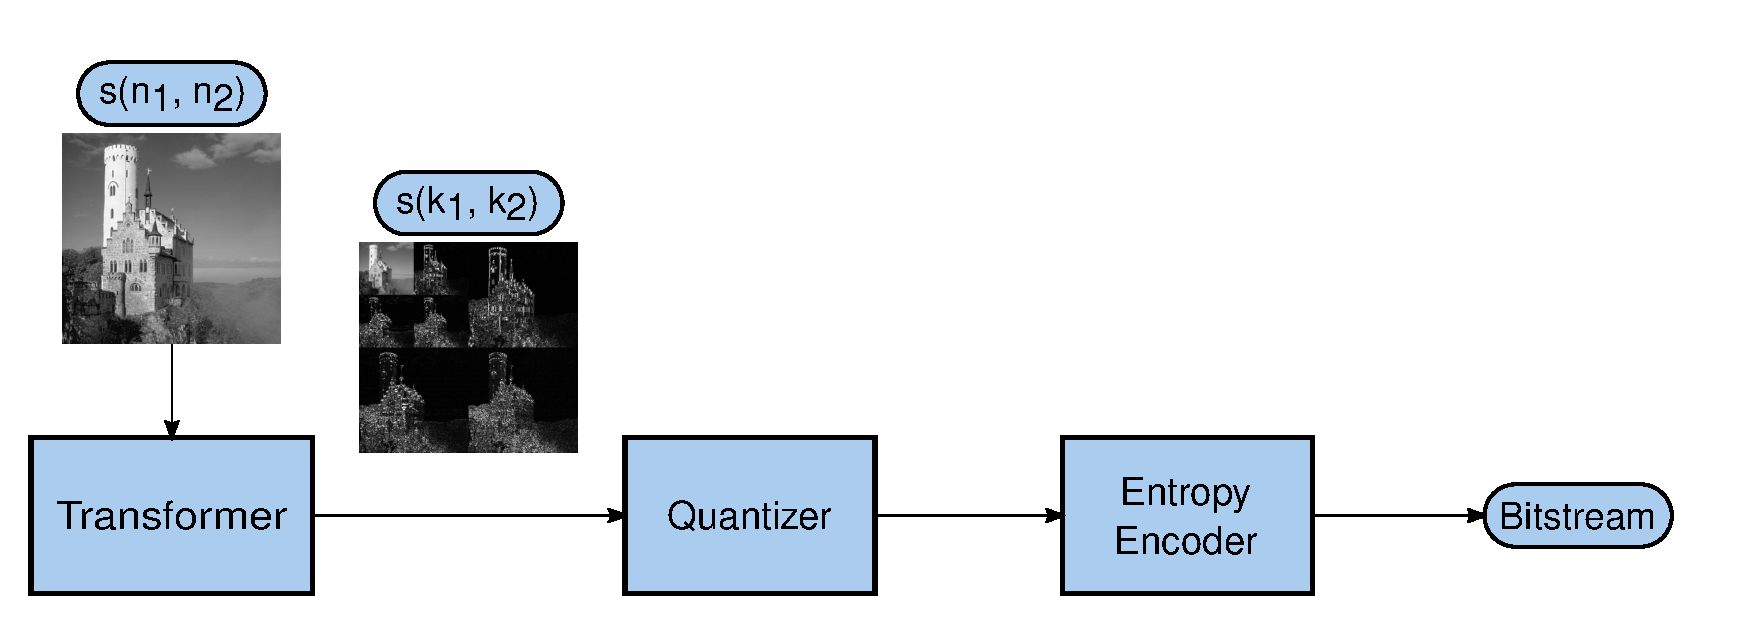
\includegraphics[scale=0.4]{../img/block-diag_shrunk.pdf}
        \caption{Transform coder: Generalised \cite{shap1993}}
    \end{figure}

    \[Quantizer \neq Quantizer\]
\end{frame}

\begin{frame}{Data compression}
    A few notable transforms include:
    \begin{itemize}
        \item Discrete Fourier Transform (DFT)
        \item Discrete Cosine Transform (DCT)
        \item Discrete Wavelet Transform (DWT)
    \end{itemize}
\end{frame}

\begin{frame}{Why choose the DWT over others?}
    \begin{itemize}
        \item The ability to truncate (stop) the encoding of bits, without
            significant loss of information
        \item DWT is more resilient to artefact formation (e.g. box artefacts)
    \end{itemize}
\end{frame}

\begin{frame}{The embedded zerotree wavelet algorithm}
    The algorithm is anchored on these key concepts: \cite{shap1993, sayood_datac}
    \vspace{0.5cm}

    \begin{enumerate}
        \item Decompose image into hierarchical sub-bands (using DWT)
        \item Exploit the fact that a single coefficient in a smaller sub-band
            may represent the same spatial location as multiple coefficients in
            \textit{other sub-bands}
        \item Successive-approximation quantization
        \item Compression using an entropy coding technique that is lossless
            such as adaptive arithmetic coding
    \end{enumerate}
\end{frame}

\begin{frame}{Limitations}
    \begin{itemize}
        \item Assumes that only a particular sub-band (\textit{LL}) is split iteratively
        \item Incapable of exploiting spatial redundancies present in
            coefficients \textit{within the same sub-band}
    \end{itemize}
\end{frame}

\section{Problem statement}
\begin{frame}{Problem statement}
    To implement the \textit{Embedded Zerotree Wavelet} algorithm for image
    compression as a C library, and study its performance under various
    circumstances.
\end{frame}

\section{Implementation approach}
\begin{frame}{Software implementation}
    \begin{itemize}
        \item External library for computing DWT \cite{wavelib}
        \item We implement the EZW algorithm on the transformed output
    \end{itemize}
\end{frame}

\section{Conclusion}
\subsection{Proposed outcomes}
\begin{frame}
    A fully operative EZW coder, with data to support claims made earlier.
\end{frame}

\subsection{Future work}
\begin{frame}
    \begin{itemize}
        \item A multi-core implementation of the algorithm
        \item An FPGA-based hardware accelerator for the algorithm
    \end{itemize}
\end{frame}

\section{References}
\begin{frame}
    \printbibliography
\end{frame}

\section{End}
\begin{frame}
    \centering
    \huge{Thank You}
    \par
    \huge{Questions?}
\end{frame}

\end{document}

